\documentclass[a4paper,12pt]{article}
	\usepackage[left=2cm,right=1cm,top=1cm,bottom=1.5cm]{geometry}
	\usepackage[utf8]{inputenc}
	\usepackage[english,russian]{babel}
	\usepackage{graphicx}
	\usepackage{listings}
	\lstset{language=SQL, extendedchars=\true}
	\usepackage{amsmath}
	\usepackage{amssymb}
	\usepackage{cite}
	\usepackage{indentfirst}
	\usepackage{multicol}
	\usepackage{cmap}
	
	\sloppy
	
	\usepackage{geometry}
	\geometry{top=2cm}
	\geometry{bottom=2cm}
	\geometry{left=2.5cm}
	\geometry{right=2.5cm}
	
	\renewcommand{\baselinestretch}{1.5}
	
\begin{document}
\renewcommand{\contentsname}{\Large Содержание}
\renewcommand{\bibname}{\normalfont\Large\bfseries Список литературы}

\begin{titlepage}
    \begin{center}
        Министерство науки и высшего образования Российской Федерации \\
        НАЦИОНАЛЬНЫЙ ИССЛЕДОВАТЕЛЬСКИЙ ЯДЕРНЫЙ УНИВЕРСИТЕТ <<МИФИ>> \\*
        \hrulefill
    \end{center}

    \begin{center}
        ИНСТИТУТ ЛАЗЕРНЫХ И ПЛАЗМЕННЫХ ТЕХНОЛОГИЙ\\
        КАФЕДРА №31 ПРИКЛАДНАЯ МАТЕМАТИКА
    \end{center}
    \vspace{1cm}

    \vspace{2em}

    \begin{center}
        \large{Отчет}

        по лабораторным работам по предмету:

        Базы данных (теоретические основы баз данных)
    \end{center}

    \begin{center}
        \textit{Выполнили: Есис А.И., Суслова И.И., группа Б20-215}

        \textit{Преподаватель: Павленко Дарья Александровна}
    \end{center}


    \vspace{31em}

    \begin{center}
        г. Москва 2022
    \end{center}
\end{titlepage}

\newpage
\tableofcontents
\setcounter{page}{3}

\newpage
\section{Введение}

\textsl{LiveLib.ru} -- русскоязычный интернет-проект, социальная сеть, посвящённая литературе. Сайт предоставляет информацию о книгах, писателях, издательствах, библиотеках, а также даёт возможность ведения читательских дневников, обсуждения книг; публикует рейтинги пользовательских предпочтений, информацию о книжных новинках и литературных новостях, произведениях и изданиях, авторах книг, издательствах и издательских серий книг, библиотеках. Основной контент сайта создается пользователями. Пользователи могут общаться на форуме, играть в различные литературные игры, участвовать в конкурсах. Также благодаря данному сервису между читателями осуществляется обмен литературой.

В рамках данной лабораторной работы из всего многообразия функционала было выделено следующее:
\begin{enumerate}
    \item Получение информации о книгах, авторах.
    \item Обмен мнениями между пользователями: возможность добавить отзыв к книге или автору, написать историю или цитату к книге, создать обсуждение, отметить книгу понравившейся, прочитанной, недочитанной и остальное. А также некоторые дополнительные функции, такие как: добавление в друзья, получение достижений за различные действия на сайте.
\end{enumerate}


\newpage
\section{Схема базы данных}

Рассмотрим основные сущности, выделенные в рамках этой работы:

\begin{enumerate}
    \item \textbf{Издательства}.
    \item \textbf{Книги}.
    \item \textbf{Авторы}.
    \item \textbf{Жанры}.
    \item \textbf{Цитаты} -- цитаты из книги, добавленные пользователями.
    \item \textbf{Истории} -- истории из жизни пользователей, связанные с той или иной книгой.
    \item \textbf{Отзывы}.
    \item \textbf{Подборки}.
    \item \textbf{Пользователи}.
    \item \textbf{Друзья}.
    \item \textbf{Достижения}.
    \item \textbf{Оценки} -- оценки к разным объектам на сайте (отзыву, цитате или истории).
    \item \textbf{Обсуждения}.
    \item \textbf{Статьи} -- сообщения пользователей в каком-либо обсуждении.
    \item \textbf{Тип отношения пользователь-книга} -- пользователь может отметить книгу понравившейся, прочитанной, перечитанной, недочитанной, "читает сейчас", "хочет прочитать".
\end{enumerate}

На Рис. \ref{fig:database_c} можно увидеть схему связей между этими сущностями -- концептуальную модель базы данных.

\begin{figure}[ht]
    \center{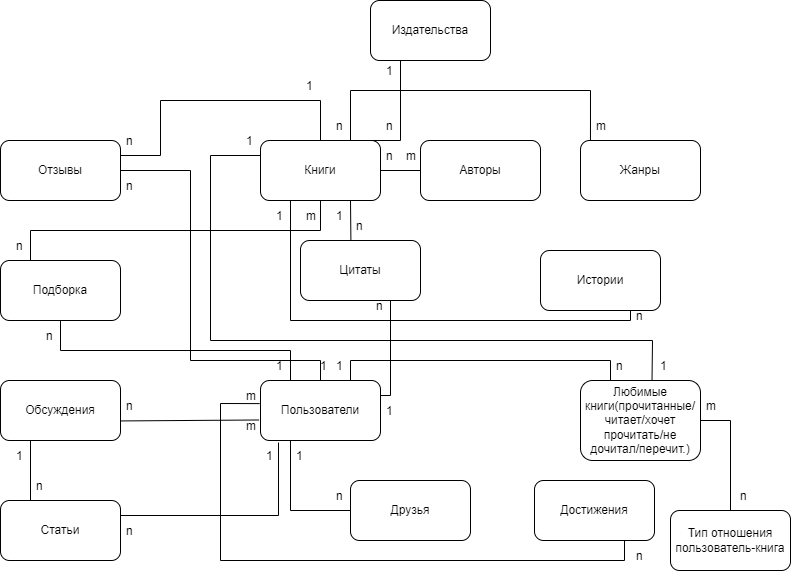
\includegraphics[scale=0.6]{LiveLib.png}}
    \caption{Концептуальная модель базы данных}
    \label{fig:database_c}
\end{figure}

Далее необходимо выделить для каждой сущности поля (поля created, deleted, updated содержат информацию о дате и времени создания, удаления и обновления записи и подразумеваются в каждой таблице):

\begin{enumerate}
    \item \textbf{source} (картинки, файлы, какие-либо ресурсы) в файловой системе): путь в файловой системе.
    \item \textbf{Издательства}: publisher\_id, название.
    \item \textbf{Книги}: book\_id, название, описание, дата выхода, publisher\_id, серия, обложка.
    \item \textbf{Авторы}: author\_id, имя, фамилия, фото, описание, годы жизни.
    \item \textbf{Книга – Автор}: book\_id, author\_id.
    \item \textbf{Жанры}: genre\_id, название.
    \item \textbf{Книга – Жанр}: book\_id, genre\_id.
    \item \textbf{Цитаты}: quotes\_id, book\_id, user\_id, текст.
    \item \textbf{Истории}: story\_id, book\_id, user\_id, текст.
    \item \textbf{Отзывы}: review\_id, book\_id, user\_id, текст, рейтинг.
    \item \textbf{Подборки}: user\_id, user\_id (автор), название, описание.
    \item \textbf{Книга – Подборка}: book\_id, list\_id.
    \item \textbf{Пользователи}: user\_id, имя, фамилия, nick, пол, описание, фото, пароль.
    \item \textbf{Друзья} (пользователь – пользователь): id, user\_id\_1, user\_id\_2.
    \item \textbf{Достижения}: reword\_id, название, картинка, описание (за что можно получить).
    \item \textbf{Достижение – пользователь}: id\_user, id\_reword.
    \item \textbf{Оценки}: mark\_id, чему оценка (отзыв, цитата, история), оценка.
    \item \textbf{Обсуждения}: dialog\_id, user\_id (автор), название, описание.
    \item \textbf{Статьи}: article\_id, user\_id (автор), dialog\_id (обсуждение), текст.
    \item \textbf{Тип отношения пользователь-книга}: user\_book\_type\_id, название.
    \item \textbf{Пользователь – Книга}: id, user\_book\_type\_id, book\_id, user\_id.
\end{enumerate}

На Рис. \ref{fig:database_l} представлена логическая модель базы данных.

\begin{figure}[]
    \center{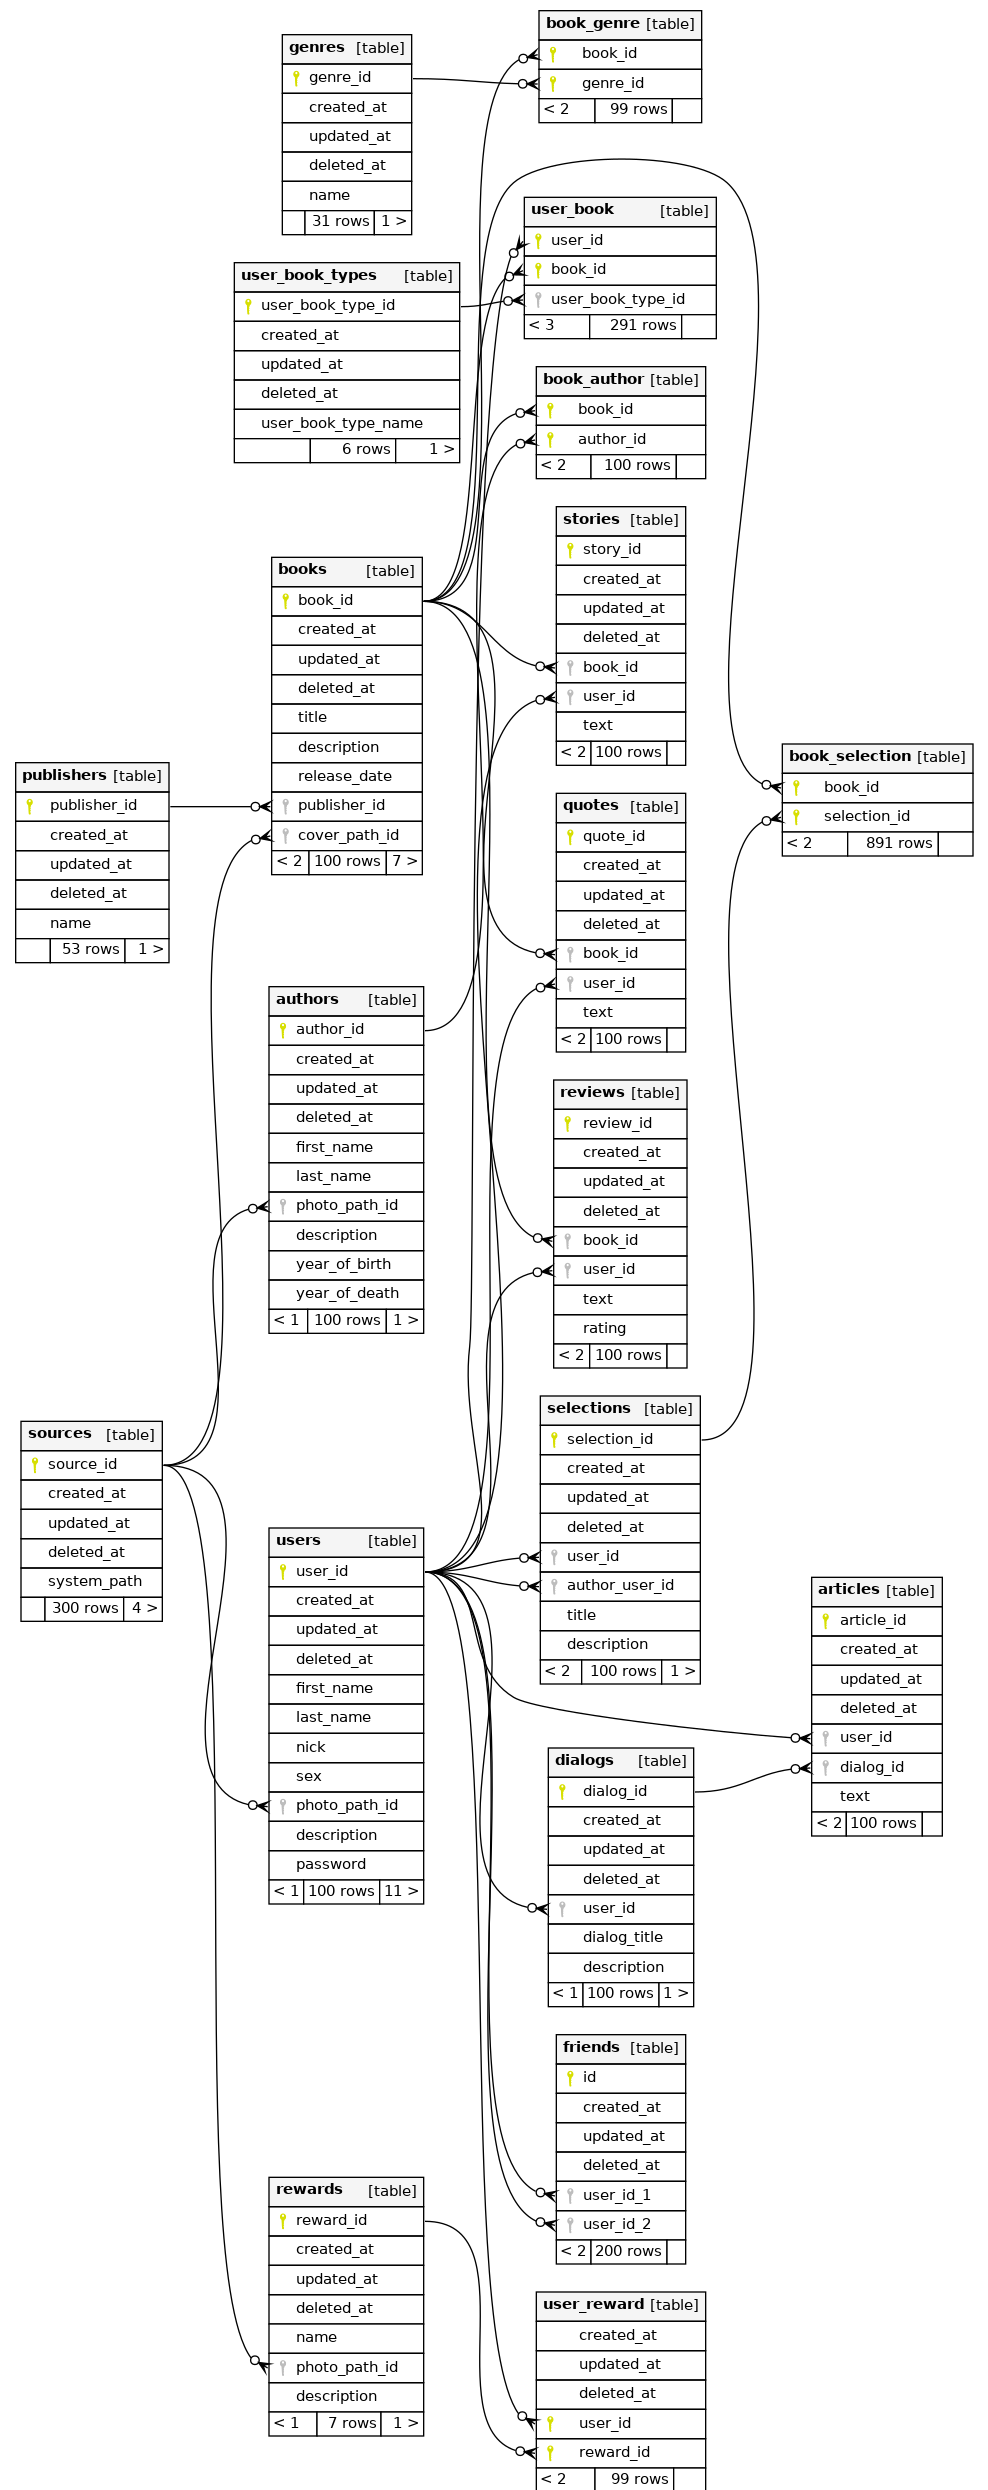
\includegraphics[scale=0.36]{relationships.png}}
    \caption{Логическая модель базы данных}
    \label{fig:database_l}
\end{figure}


\newpage
\section{Создание базы данных}
В соответствии со схемой был написан следующий \emph{create}-запрос:
\begin{lstlisting}
CREATE TABLE IF NOT EXISTS "sources" (
    source_id INT GENERATED ALWAYS AS IDENTITY PRIMARY KEY,
    created_at TIMESTAMPTZ DEFAULT CURRENT_TIMESTAMP NOT NULL,
    updated_at TIMESTAMPTZ DEFAULT CURRENT_TIMESTAMP NOT NULL,
    deleted_at TIMESTAMPTZ DEFAULT NULL,
    system_path TEXT NOT NULL
);
------------------------------------------------------------------
CREATE TABLE IF NOT EXISTS "publishers" (
    publisher_id INT GENERATED ALWAYS AS IDENTITY PRIMARY KEY,
    created_at TIMESTAMPTZ DEFAULT CURRENT_TIMESTAMP NOT NULL,
    updated_at TIMESTAMPTZ DEFAULT CURRENT_TIMESTAMP NOT NULL,
    deleted_at TIMESTAMPTZ NULL,
    name VARCHAR(128) UNIQUE NOT NULL
);
-----------------------------------------------------------------
CREATE TABLE IF NOT EXISTS "books" (
    book_id INT GENERATED ALWAYS AS IDENTITY PRIMARY KEY,
    created_at TIMESTAMPTZ DEFAULT CURRENT_TIMESTAMP NOT NULL,
    updated_at TIMESTAMPTZ DEFAULT CURRENT_TIMESTAMP NOT NULL,
    deleted_at TIMESTAMPTZ DEFAULT NULL,
    title VARCHAR(256) NOT NULL,
    description TEXT DEFAULT NULL,
    release_date TIMESTAMPTZ NOT NULL,
    publisher_id INT NOT NULL,
    CONSTRAINT publisher_fk FOREIGN KEY(publisher_id) REFERENCES
        publishers(publisher_id) ON DELETE SET NULL,
    cover_path_id INT NOT NULL,
    CONSTRAINT cover_fk FOREIGN KEY(cover_path_id) REFERENCES
        sources(source_id) ON DELETE SET NULL
);
--------------------------------------------------------
CREATE TABLE IF NOT EXISTS "authors" (
    author_id INT GENERATED ALWAYS AS IDENTITY PRIMARY KEY,
    created_at TIMESTAMPTZ DEFAULT CURRENT_TIMESTAMP NOT NULL,
    updated_at TIMESTAMPTZ DEFAULT CURRENT_TIMESTAMP NOT NULL,
    deleted_at TIMESTAMPTZ DEFAULT NULL,
    first_name VARCHAR(128) NOT NULL,
    last_name VARCHAR(128) NOT NULL,
    photo_path_id INT DEFAULT NULL,
    CONSTRAINT photo_path_fk FOREIGN KEY(photo_path_id) REFERENCES
        sources(source_id) ON DELETE SET NULL,
    description TEXT DEFAULT NULL,
    year_of_birth TIMESTAMPTZ NOT NULL,
    year_of_death TIMESTAMPTZ DEFAULT NULL
);
------------------------------------------------------------------
CREATE TABLE IF NOT EXISTS "book_author" (
    book_id INT REFERENCES books(book_id) ON UPDATE CASCADE ON DELETE 
        SET NULL,
    author_id INT REFERENCES authors(author_id) ON UPDATE CASCADE,
    CONSTRAINT book_author_pk PRIMARY KEY (book_id, author_id)
);
------------------------------------------------------------------
CREATE TABLE IF NOT EXISTS "genres" (
    genre_id INT GENERATED ALWAYS AS IDENTITY PRIMARY KEY,
    created_at TIMESTAMPTZ DEFAULT CURRENT_TIMESTAMP NOT NULL,
    updated_at TIMESTAMPTZ DEFAULT CURRENT_TIMESTAMP NOT NULL,
    deleted_at TIMESTAMPTZ DEFAULT NULL,
    name VARCHAR(128) UNIQUE NOT NULL
);
----------------------------------------------------------------
CREATE TABLE IF NOT EXISTS "book_genre" (
    book_id INT REFERENCES books(book_id) ON UPDATE CASCADE ON DELETE 
        SET NULL,
    genre_id INT REFERENCES genres(genre_id) ON UPDATE CASCADE,
    CONSTRAINT book_genre_pk PRIMARY KEY (book_id, genre_id)
);
----------------------------------------------------------------
CREATE TABLE IF NOT EXISTS "users" (
    user_id INT GENERATED ALWAYS AS IDENTITY PRIMARY KEY,
    created_at TIMESTAMPTZ DEFAULT CURRENT_TIMESTAMP NOT NULL,
    updated_at TIMESTAMPTZ DEFAULT CURRENT_TIMESTAMP NOT NULL,
    deleted_at TIMESTAMPTZ DEFAULT NULL,
    first_name VARCHAR(128) NOT NULL,
    last_name VARCHAR(128) NOT NULL,
    nick VARCHAR(128) NOT NULL,
    sex VARCHAR(6) DEFAULT NULL,
    photo_path_id INT DEFAULT NULL,
    CONSTRAINT photo_path_fk FOREIGN KEY(photo_path_id) REFERENCES
        sources(source_id) ON DELETE SET NULL,
    description TEXT DEFAULT NULL,
    password VARCHAR(128) NOT NULL
);
----------------------------------------------------------------
CREATE TABLE IF NOT EXISTS "quotes" (
    quote_id INT GENERATED ALWAYS AS IDENTITY PRIMARY KEY,
    created_at TIMESTAMPTZ DEFAULT CURRENT_TIMESTAMP NOT NULL,
    updated_at TIMESTAMPTZ DEFAULT CURRENT_TIMESTAMP NOT NULL,
    deleted_at TIMESTAMPTZ DEFAULT NULL,
    book_id INT,
    CONSTRAINT book_fk FOREIGN KEY(book_id) REFERENCES books(book_id) 
        ON DELETE SET NULL,
    user_id INT,
    CONSTRAINT user_fk FOREIGN KEY(user_id) REFERENCES users(user_id) 
        ON DELETE SET NULL,
    text TEXT NOT NULL
);
---------------------------------------------------------------------
CREATE TABLE IF NOT EXISTS "stories" (
    story_id INT GENERATED ALWAYS AS IDENTITY PRIMARY KEY,
    created_at TIMESTAMPTZ DEFAULT CURRENT_TIMESTAMP NOT NULL,
    updated_at TIMESTAMPTZ DEFAULT CURRENT_TIMESTAMP NOT NULL,
    deleted_at TIMESTAMPTZ DEFAULT NULL,
    book_id INT NOT NULL,
    CONSTRAINT book_fk FOREIGN KEY(book_id) REFERENCES books(book_id) 
        ON DELETE CASCADE,
    user_id INT NOT NULL,
    CONSTRAINT user_fk FOREIGN KEY(user_id) REFERENCES users(user_id) 
        ON DELETE CASCADE,
    text TEXT NOT NULL
);
---------------------------------------------------------------------
CREATE TABLE IF NOT EXISTS "reviews" (
    review_id INT GENERATED ALWAYS AS IDENTITY PRIMARY KEY,
    created_at TIMESTAMPTZ DEFAULT CURRENT_TIMESTAMP NOT NULL,
    updated_at TIMESTAMPTZ DEFAULT CURRENT_TIMESTAMP NOT NULL,
    deleted_at TIMESTAMPTZ DEFAULT NULL,
    book_id INT NOT NULL,
    CONSTRAINT book_fk FOREIGN KEY(book_id) REFERENCES books(book_id) 
        ON DELETE CASCADE,
    user_id INT NOT NULL,
    CONSTRAINT user_fk FOREIGN KEY(user_id) REFERENCES users(user_id) 
        ON DELETE CASCADE,
    text TEXT NOT NULL,
    rating SMALLINT NOT NULL,
    CONSTRAINT rating_from_0_to_5 CHECK (
        rating >= 0
        AND rating <= 5
    )
);
----------------------------------------------------------------
CREATE TABLE IF NOT EXISTS "friends" (
    id INT GENERATED ALWAYS AS IDENTITY PRIMARY KEY,
    created_at TIMESTAMPTZ DEFAULT CURRENT_TIMESTAMP NOT NULL,
    updated_at TIMESTAMPTZ DEFAULT CURRENT_TIMESTAMP NOT NULL,
    deleted_at TIMESTAMPTZ DEFAULT NULL,
    user_id_1 INT REFERENCES users(user_id) ON UPDATE CASCADE 
        ON DELETE SET NULL,
    user_id_2 INT REFERENCES users(user_id) ON UPDATE CASCADE
);
----------------------------------------------------------------
CREATE TABLE IF NOT EXISTS "rewards" (
    reward_id INT GENERATED ALWAYS AS IDENTITY PRIMARY KEY,
    created_at TIMESTAMPTZ DEFAULT CURRENT_TIMESTAMP NOT NULL,
    updated_at TIMESTAMPTZ DEFAULT CURRENT_TIMESTAMP NOT NULL,
    deleted_at TIMESTAMPTZ DEFAULT NULL,
    name VARCHAR(128) UNIQUE NOT NULL,
    photo_path_id INT DEFAULT NULL,
    CONSTRAINT photo_path_fk FOREIGN KEY(photo_path_id) 
        REFERENCES sources(source_id) ON DELETE SET NULL,
    description TEXT DEFAULT NULL
);
----------------------------------------------------------------
CREATE TABLE user_reward (
    created_at TIMESTAMPTZ DEFAULT CURRENT_TIMESTAMP NOT NULL,
    updated_at TIMESTAMPTZ DEFAULT CURRENT_TIMESTAMP NOT NULL,
    deleted_at TIMESTAMPTZ DEFAULT NULL,
    user_id INT REFERENCES users(user_id) ON UPDATE CASCADE ON DELETE 
        SET NULL,
    reward_id INT REFERENCES rewards(reward_id) ON UPDATE CASCADE,
    CONSTRAINT user_reward_pk PRIMARY KEY (user_id, reward_id)
);
----------------------------------------------------------------
CREATE TABLE IF NOT EXISTS "user_book_types" (
    user_book_type_id INT GENERATED ALWAYS AS IDENTITY PRIMARY KEY,
    created_at TIMESTAMPTZ DEFAULT CURRENT_TIMESTAMP NOT NULL,
    updated_at TIMESTAMPTZ DEFAULT CURRENT_TIMESTAMP NOT NULL,
    deleted_at TIMESTAMPTZ DEFAULT NULL,
    user_book_type_name VARCHAR(128) UNIQUE NOT NULL
);
--------------------------------------------------------------------
CREATE TABLE IF NOT EXISTS "marks" (
    mark_id INT GENERATED ALWAYS AS IDENTITY PRIMARY KEY,
    created_at TIMESTAMPTZ DEFAULT CURRENT_TIMESTAMP NOT NULL,
    updated_at TIMESTAMPTZ DEFAULT CURRENT_TIMESTAMP NOT NULL,
    deleted_at TIMESTAMPTZ DEFAULT NULL,
    type_of_marked_object VARCHAR(128) NOT NULL,
    value_of_mark INT DEFAULT 0 NOT NULL,
    CONSTRAINT value_of_mark_from_0_to_5 CHECK (
        value_of_mark >= 0
        AND value_of_mark <= 5
    )
);
----------------------------------------------------------------
CREATE TABLE IF NOT EXISTS "dialogs" (
    dialog_id INT GENERATED ALWAYS AS IDENTITY PRIMARY KEY,
    created_at TIMESTAMPTZ DEFAULT CURRENT_TIMESTAMP NOT NULL,
    updated_at TIMESTAMPTZ DEFAULT CURRENT_TIMESTAMP NOT NULL,
    deleted_at TIMESTAMPTZ DEFAULT NULL,
    user_id INT NOT NULL,
    CONSTRAINT user_id_fk FOREIGN KEY(user_id) REFERENCES 
        users(user_id) ON DELETE SET NULL,
    dialog_title VARCHAR(128) NOT NULL,
    description TEXT DEFAULT NULL
);
--------------------------------------------------------------------
CREATE TABLE IF NOT EXISTS "selections" (
    selection_id INT GENERATED ALWAYS AS IDENTITY PRIMARY KEY,
    created_at TIMESTAMPTZ DEFAULT CURRENT_TIMESTAMP NOT NULL,
    updated_at TIMESTAMPTZ DEFAULT CURRENT_TIMESTAMP NOT NULL,
    deleted_at TIMESTAMPTZ DEFAULT NULL,
    user_id INT NOT NULL,
    CONSTRAINT user_fk FOREIGN KEY(user_id) REFERENCES users(user_id) 
        ON DELETE CASCADE,
    author_user_id INT NOT NULL,
    CONSTRAINT author_user_fk FOREIGN KEY(author_user_id) REFERENCES
        users(user_id) ON DELETE CASCADE,
    title TEXT NOT NULL,
    description TEXT NOT NULL
);
------------------------------------------------------------------
CREATE TABLE IF NOT EXISTS "book_selection" (
    book_id INT REFERENCES books(book_id) ON UPDATE CASCADE ON DELETE
        CASCADE,
    selection_id INT REFERENCES selections(selection_id) ON UPDATE
        CASCADE,
    CONSTRAINT book_selection_pk PRIMARY KEY (book_id, selection_id)
);
----------------------------------------------------------------
CREATE TABLE IF NOT EXISTS "articles" (
    article_id INT GENERATED ALWAYS AS IDENTITY PRIMARY KEY,
    created_at TIMESTAMPTZ DEFAULT CURRENT_TIMESTAMP NOT NULL,
    updated_at TIMESTAMPTZ DEFAULT CURRENT_TIMESTAMP NOT NULL,
    deleted_at TIMESTAMPTZ DEFAULT NULL,
    user_id INT NOT NULL,
    CONSTRAINT user_id_fk FOREIGN KEY(user_id) REFERENCES users(user_id)
        ON DELETE SET NULL,
    dialog_id INT NOT NULL,
    CONSTRAINT dialog_id_fk FOREIGN KEY(dialog_id) REFERENCES
        dialogs(dialog_id) ON DELETE SET NULL,
    text TEXT DEFAULT NULL
);
----------------------------------------------------------------
CREATE TABLE "user_book" (
    user_id INT REFERENCES users(user_id) ON UPDATE CASCADE 
        ON DELETE SET NULL,
    book_id INT REFERENCES books(book_id) ON UPDATE CASCADE 
        ON DELETE SET NULL,
    CONSTRAINT user_book_pk PRIMARY KEY (user_id, book_id),
    user_book_type_id INT,
    CONSTRAINT user_book_type_id_fk FOREIGN KEY(user_book_type_id)
        REFERENCES user_book_types(user_book_type_id) ON DELETE SET NULL
);
    \end{lstlisting}

\newpage
\section{Генерация данных}
Для генерации данных была использована библиотека для \textsl{Python}: \textsl{mimesis}, позволяющая сгенерировать случайные имена, ники, даты, а также слова, предложения, цитаты. Рассмотрим несколько примеров генерации данных.

Генерация названий \textbf{файлов}:
\begin{lstlisting}[language=Python]
n = 300
import random

sources = []
root = "root/"
extentions = [".jpg", ".png"]
def to_path(i):
  current = i
  path = ""
  cnt = 0;
  while current != 0:
    path += chr(current % (ord('z') - ord('a') + 1) + ord('a'))
    current //= (ord('z') - ord('a') + 1)
    cnt += 1
    if cnt == 1:
      path += '/'
    elif (cnt - 1) % 3  == 0:
      path += '/'
  while cnt < 7:
    path += 'a'
    cnt += 1
    if (cnt - 1) % 3  == 0:
      path += '/'
  return path[::-1]

for i in range(n):
  sources += [root[:-1] + to_path(i) +
        extentions[random.randint(0, len(extentions) - 1)]]
    \end{lstlisting}

Данный код сгенерирует данные в следующем виде:
\begin{lstlisting}[language=Python]
'root/aaa/aaa/a.jpg'
'root/aaa/aaa/b.jpg'
'root/aaa/aaa/c.png'
'root/aaa/aaa/d.jpg'
'root/aaa/aaa/e.jpg'
...
'root/aaa/aab/a.png'
'root/aaa/aab/b.jpg'
...
    \end{lstlisting}

Данный способ позволяет сохранить до $26^7$ объектов.

Генерация \textbf{цитат}. Генерация отзывов, историй, статей осуществляется похожим образом.

\begin{lstlisting}[language=Python]
n = 100
min_sentences = 3
max_sentences = 15

import random
from mimesis import locales
from mimesis import Text

text = Text('ru')

quotes = []
for i in range(n):
    quotes.append(text.quote())
quotes[:min(n, 1)]
    \end{lstlisting}

Цитаты создаются при помощи библиотеки \emph{mimesis}, которая предоставляет случайную цитату при вызове соответствующей функции. Для отзывов и других текстовых полей используется функция для получения случайных предложений (пример далее, в генерации описания для пользователя).

Генерация \textbf{пользователей}:

\begin{lstlisting}[language=Python]
min_sentences = 0
max_sentences = 3

from mimesis import locales, enums
from mimesis import Generic
import random
import hashlib

class User:
    def __init__(self):
        generic = Generic('ru')
        self.sex = random.choice([enums.Gender.MALE,
            enums.Gender.FEMALE])
        self.name = generic.person.name(gender=self.sex)
        self.last_name = generic.person.last_name(gender=self.sex)
        self.nick = generic.person.username()
        self.description = generic.text.text(quantity=random
            .randint(min_sentences, max_sentences))
        self.photo = random.choice(sources) 
        self.password = hashlib.md5(generic.person.password()
            .encode('utf-8')).hexdigest()
        self.sex = 'male' if self.sex == enums.Gender.MALE 
            else 'female'
    \end{lstlisting}

Данный код, при создании класса \emph{User} создает один объект, заполненный необходимыми данными. Как видно из кода, пол определяется случайным выбором, далее в соответствии с полом генерируются русские имя и фамилия (так как сайт является русскоязычным), ник, описание (несколько случайных предложений в случайном количестве от 0 до 3). Фото является случайным элементом из списка ресурсов. Пароль храниться в виде хэша (\emph{md-5}) от случайного пароля, сгенерированного библиотекой. Генерация авторов происходит аналогично.

Ряд полей (названия издательств, названия книг, типы отношения пользователь-книга были заполнены осмысленными данными вручную). Например, \textbf{достижения}:

\begin{lstlisting}[language=Python]
import random

class Reward:
    def __init__(this, name, description):
        this.name = name
        this.source = random.choice(sources)
        this.description = description
    def __str__(this):
        return ' '.join([this.name, this.source, this.description])

rewards = [Reward("Книгочей", "1500+ прочитанных книг"),
           Reward("Критик", "30+ рецензий с оценкой 50+"),
           Reward("Цитатчик", "1000+ цитат"),
           Reward("Комментатор", "3000+ комментариев"),
           Reward("Большой друг", "250+ взаимных друзей"),
           Reward("Рассказчик", "5 историй с оценкой 50+"),
           Reward("Старожил",  
                "1000 дней на сайте, 100+ прочитанных книг"),
           ]
    \end{lstlisting}

Названия и описание были взяты с сайта.

Сгенерированные данные были добавлены в соответствующую таблицу. Пример подключения и \emph{insert}-запроса:
\begin{lstlisting}[language=Python]
import psycopg2

conn = psycopg2.connect(database="lab",
                        host="localhost",
                        user="lab",
                        password="1111",
                        port="5432")

cursor = conn.cursor()
SQL = '''INSERT INTO books (
         title,
         description,
         release_date,
         publisher_id,
         cover_path_id
     )
 VALUES (
         'Martin Eden',
         'The title character becomes a writer, hoping to acquire 
         the respectability sought by his society-girl sweetheart.',
         '1909-09-22 00:00:00-00',
         1,
         1
     );
cursor.execute(SQL)
conn.commit()
    \end{lstlisting}


\newpage
\section{Примеры запросов}
Далее рассмотрим ряд запросов к данной базе для получения необходимой информации.

\underline{Запрос 1}. \textbf{Получение всех имен друзей пользователей}.
\begin{lstlisting}
SELECT u1.first_name,
    u1.last_name,
    u2.first_name,
    u2.last_name
FROM friends
    JOIN users u1 on u1.user_id = friends.user_id_1
    JOIN users u2 on u2.user_id = friends.user_id_2
ORDER BY u1.first_name;
    \end{lstlisting}

\textbf{Результат} (несколько первых записей) -- Рис. \ref{fig:request1}.

\begin{figure}[ht]
    \center{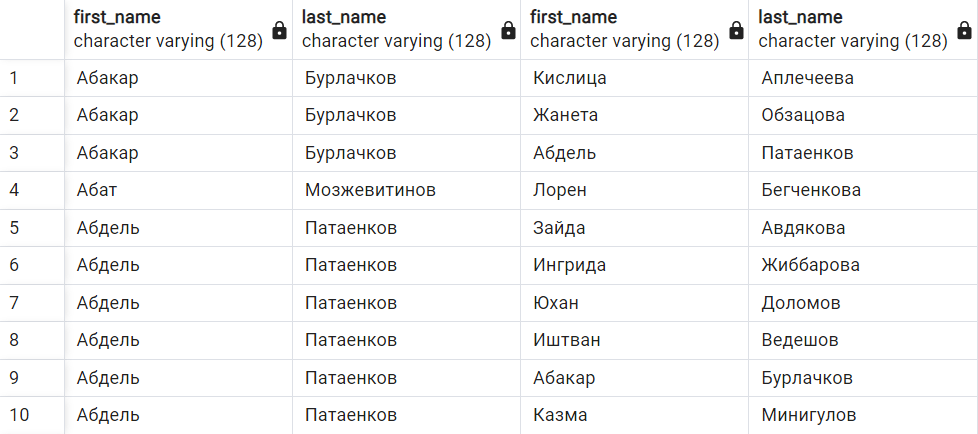
\includegraphics[scale=0.6]{request1.png}}
    \caption{Результат выполнения запроса 1.}
    \label{fig:request1}
\end{figure}

\underline{Запрос 2}. \textbf{Получение пользователей, у которых больше трёх друзей}.
\begin{lstlisting}
SELECT u1.first_name,
    u1.last_name,
    COUNT(u2.nick)
FROM friends
    JOIN users u1 on u1.user_id = friends.user_id_1
    JOIN users u2 on u2.user_id = friends.user_id_2
GROUP BY u1.first_name,
    u1.last_name
HAVING COUNT(u2.nick) >= 4
ORDER BY COUNT(u2.nick) DESC;
    \end{lstlisting}

\textbf{Результат} (несколько первых записей) -- Рис. \ref{fig:request2}.

\begin{figure}[ht]
    \center{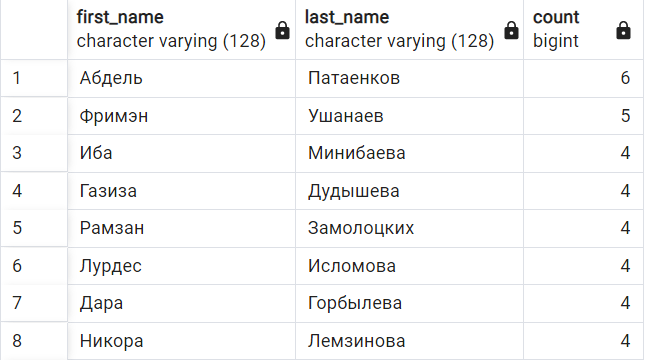
\includegraphics[scale=0.6]{request2.png}}
    \caption{Результат выполнения запроса 2.}
    \label{fig:request2}
\end{figure}

\underline{Запрос 3}. \textbf{Получение информации о книге -- название, автор, издательство}.
\begin{lstlisting}
SELECT b.title,
    a.first_name,
    a.last_name,
    p.name
FROM book_author
    JOIN authors a on a.author_id = book_author.author_id
    JOIN books b on b.book_id = book_author.book_id
    JOIN publishers p on p.publisher_id = b.publisher_id;
    \end{lstlisting}

\textbf{Результат} (несколько первых записей) -- Рис. \ref{fig:request3}.

\begin{figure}[ht]
    \center{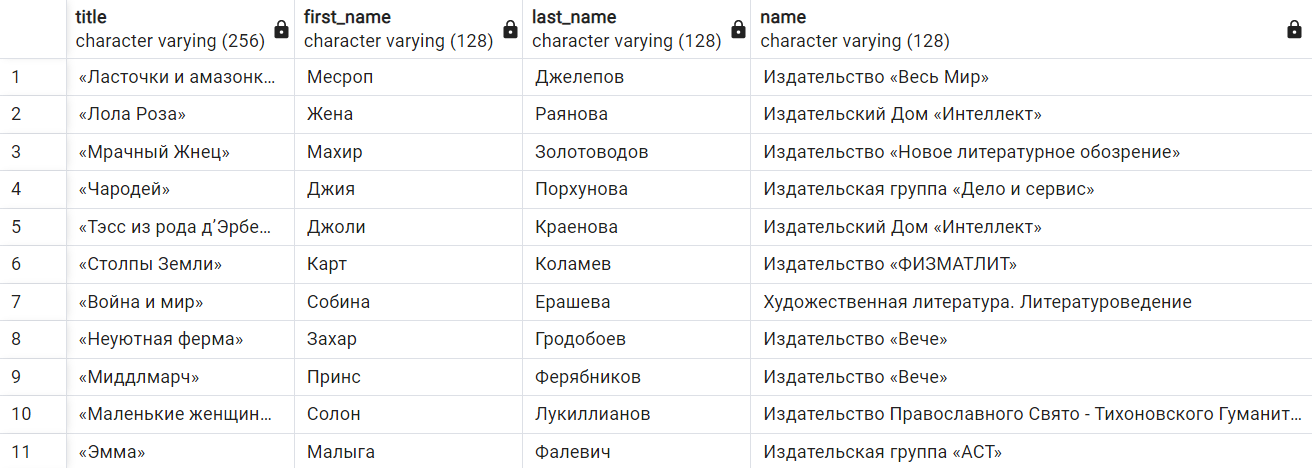
\includegraphics[scale=0.5]{request3.png}}
    \caption{Результат выполнения запроса 3.}
    \label{fig:request3}
\end{figure}

\underline{Запрос 4}. \textbf{Получение автора, прожившего дольше всех}.
\begin{lstlisting}
SELECT a.first_name,
    a.last_name,
    a.year_of_birth,
    a.year_of_death,
    (a.year_of_death - a.year_of_birth) as years
FROM authors a
WHERE a.year_of_death IS NOT NULL
ORDER BY years DESC;
    \end{lstlisting}

\textbf{Результат} (несколько первых записей) -- Рис. \ref{fig:request4}.

\begin{figure}[ht]
    \center{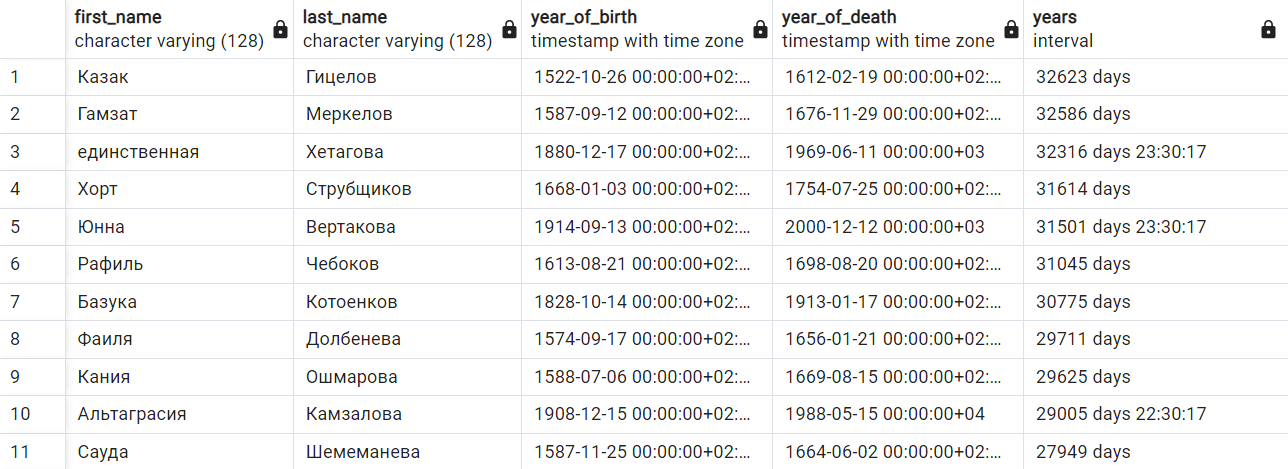
\includegraphics[scale=0.5]{request4.png}}
    \caption{Результат выполнения запроса 4.}
    \label{fig:request4}
\end{figure}

\underline{Запрос 5}. \textbf{Получение самого взрослого автора}.
\begin{lstlisting}
SELECT a.first_name,
    a.last_name,
    a.year_of_birth,
    (now() - a.year_of_birth) as years
FROM authors a
WHERE a.year_of_death IS NULL
ORDER BY years DESC;
    \end{lstlisting}

\textbf{Результат} -- Рис. \ref{fig:request5}.

\begin{figure}[ht]
    \center{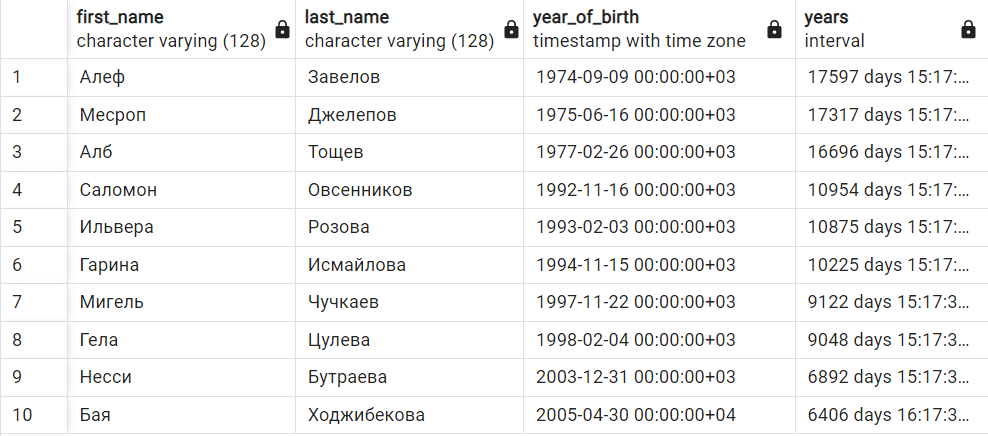
\includegraphics[scale=0.6]{request5.png}}
    \caption{Результат выполнения запроса 5.}
    \label{fig:request5}
\end{figure}

\underline{Запрос 6}. \textbf{Получение информации о количестве сколько книг прочитал}.
\begin{lstlisting}
SELECT u.first_name,
    u.last_name,
    u.nick,
    COUNT(user_book.book_id)
FROM user_book
    JOIN user_book_types ubt on 
        ubt.user_book_type_id = user_book.user_book_type_id
    JOIN users u on user_book.user_id = u.user_id
WHERE ubt.user_book_type_name = 'Прочитал(а)'
GROUP BY u.user_id
ORDER BY COUNT(user_book.book_id) DESC;
    \end{lstlisting}

\textbf{Результат} (несколько первых записей) -- Рис. \ref{fig:request6}.

\begin{figure}[ht]
    \center{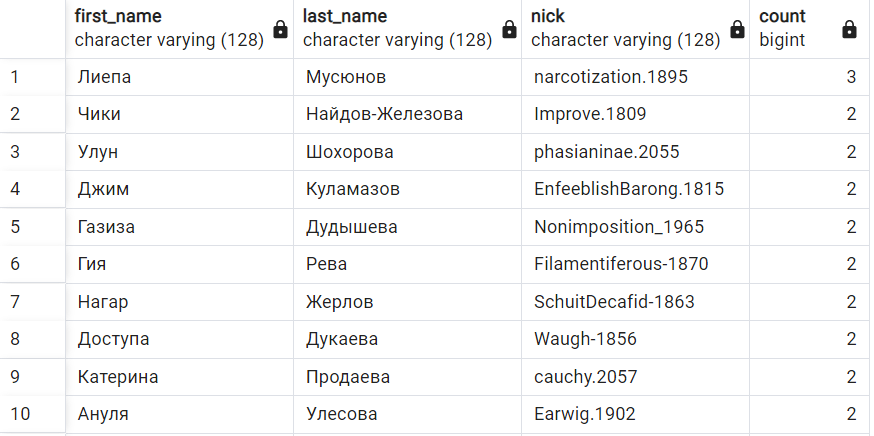
\includegraphics[scale=0.6]{request6.png}}
    \caption{Результат выполнения запроса 6.}
    \label{fig:request6}
\end{figure}

Далее рассмотрим последовательно несколько запросов, чтобы получить информацию о книгах, прочитанных только женщинами.

\underline{Запрос 7}. \textbf{Получение информации о поле людей, прочитавших какие-либо книги}.
\begin{lstlisting}
SELECT ub.user_id,
    ub.book_id,
    b.title,
    u.sex
FROM user_book AS ub
    JOIN books b on b.book_id = ub.book_id
    JOIN users u on ub.user_id = u.user_id
    JOIN user_book_types ubt on 
        ub.user_book_type_id = ubt.user_book_type_id
    JOIN book_genre bg on bg.book_id = b.book_id
    JOIN genres g on g.genre_id = bg.genre_id
WHERE g.name = 'Бизнес-книги'
    AND ubt.user_book_type_name = 'Прочитал(а)';
    \end{lstlisting}

\textbf{Результат} -- Рис. \ref{fig:request7}.

\begin{figure}[ht]
    \center{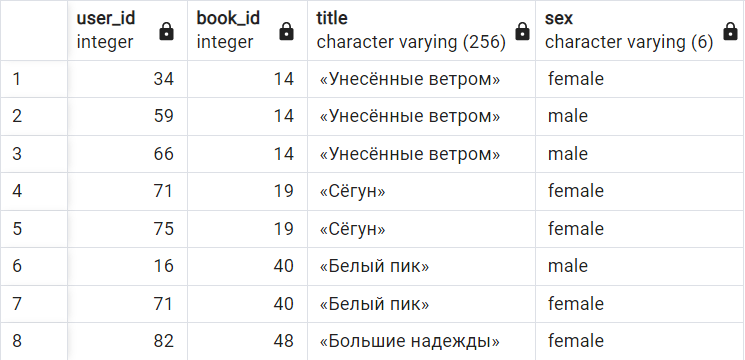
\includegraphics[scale=0.6]{request7.png}}
    \caption{Результат выполнения запроса 7.}
    \label{fig:request7}
\end{figure}

\underline{Запрос 8}. \textbf{Получение книг, которые прочитал хотя бы один мужчина}.
\begin{lstlisting}
WITH r1 AS (
    SELECT ub.user_id,
        ub.book_id,
        b.title,
        u.sex
    FROM user_book AS ub
        JOIN books b on b.book_id = ub.book_id
        JOIN users u on ub.user_id = u.user_id
        JOIN user_book_types ubt on 
            ub.user_book_type_id = ubt.user_book_type_id
        JOIN book_genre bg on bg.book_id = b.book_id
        JOIN genres g on g.genre_id = bg.genre_id
    WHERE g.name = 'Бизнес-книги'
        AND ubt.user_book_type_name = 'Прочитал(а)'
)
SELECT DISTINCT r1.title
FROM r1
    JOIN r1 r2 on r1.book_id = r2.book_id
WHERE r1.sex = 'male'
    OR r2.sex = 'male';
    \end{lstlisting}

\textbf{Результат} -- Рис. \ref{fig:request8}.

\begin{figure}[ht]
    \center{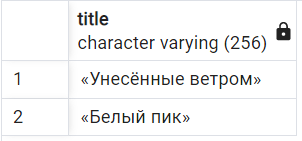
\includegraphics[scale=0.6]{request8.png}}
    \caption{Результат выполнения запроса 8.}
    \label{fig:request8}
\end{figure}

\underline{Запрос 9}. \textbf{Получение названий книг, прочитанных только женщинами}.
\begin{lstlisting}
WITH r1 AS (
    SELECT ub.user_id,
        ub.book_id,
        b.title,
        u.sex
    FROM user_book AS ub
        JOIN books b on b.book_id = ub.book_id
        JOIN users u on ub.user_id = u.user_id
        JOIN user_book_types ubt on 
            ub.user_book_type_id = ubt.user_book_type_id
        JOIN book_genre bg on bg.book_id = b.book_id
        JOIN genres g on g.genre_id = bg.genre_id
    WHERE g.name = 'Бизнес-книги'
        AND ubt.user_book_type_name = 'Прочитал(а)'
)
SELECT DISTINCT b.title
FROM user_book AS ub
    JOIN books b on b.book_id = ub.book_id
    JOIN users u on ub.user_id = u.user_id
    JOIN user_book_types ubt on 
        ub.user_book_type_id = ubt.user_book_type_id
    JOIN book_genre bg on bg.book_id = b.book_id
    JOIN genres g on g.genre_id = bg.genre_id
WHERE g.name = 'Бизнес-книги'
    AND ubt.user_book_type_name = 'Прочитал(а)'
EXCEPT
SELECT DISTINCT r1.title
FROM r1
    JOIN r1 r2 on r1.book_id = r2.book_id
WHERE r1.sex = 'male'
    OR r2.sex = 'male';
    \end{lstlisting}

\textbf{Результат} -- Рис. \ref{fig:request9}.

\begin{figure}[ht]
    \center{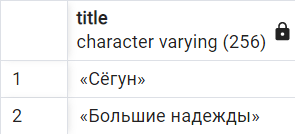
\includegraphics[scale=0.6]{request9.png}}
    \caption{Результат выполнения запроса 9.}
    \label{fig:request9}
\end{figure}

\underline{Запрос 10}. \textbf{Выделение категорий (по количеству прочитанных книг}.
\begin{lstlisting}
SELECT u.first_name,
       u.last_name,
       u.nick,
       COUNT(user_book.book_id) as books,
       CASE WHEN COUNT(user_book.book_id) BETWEEN 0 AND 1 THEN
                'мало (<=1)'
            WHEN COUNT(user_book.book_id) BETWEEN 1 AND 2 THEN
                'средне (<=2)'
            WHEN COUNT(user_book.book_id) >= 3 THEN
                'много (>=3)'
           END CASE
FROM user_book
    JOIN user_book_types ubt on 
        ubt.user_book_type_id = user_book.user_book_type_id
    JOIN users u on user_book.user_id = u.user_id
WHERE ubt.user_book_type_name = 'Прочитал(а)'
GROUP BY u.user_id
ORDER BY books DESC;
    \end{lstlisting}

\textbf{Результат} (несколько первых записей) -- Рис. \ref{fig:request10}.

\begin{figure}[ht]
    \center{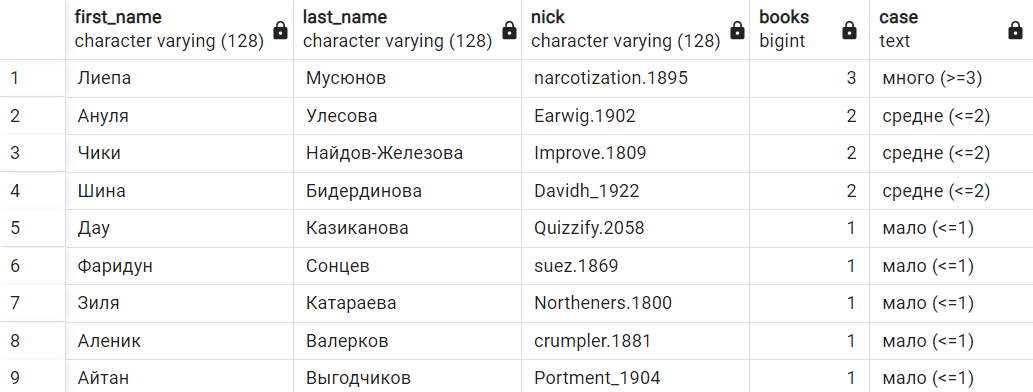
\includegraphics[scale=0.6]{request10.png}}
    \caption{Результат выполнения запроса 10.}
    \label{fig:request10}
\end{figure}

\underline{Запрос 11}. \textbf{Рекурсивный поиск друзей.}
\begin{lstlisting}
    WITH RECURSIVE r AS (SELECT user_id, nick, 1 AS level
    FROM users
    WHERE user_id = 1

    UNION ALL

    SELECT u.user_id, u.nick, r.level + 1 AS level
    FROM friends f
             JOIN r ON f.user_id_1 = r.user_id
             JOIN users u on u.user_id = f.user_id_2
    WHERE r.level < 5)
SELECT DISTINCT nick, user_id, MIN(level) as level FROM r
GROUP BY nick, user_id;
    \end{lstlisting}

\textbf{Результат} (несколько первых записей) -- Рис. \ref{fig:request11}.

\begin{figure}[ht]
    \center{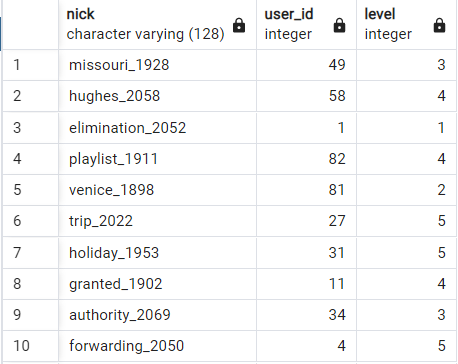
\includegraphics[scale=0.6]{request11.png}}
    \caption{Результат выполнения запроса 11.}
    \label{fig:request11}
\end{figure}

\underline{Запрос 12}. \textbf{Теория 5 рукопожатий.}
\begin{lstlisting}
    WITH RECURSIVE r AS (SELECT user_id, nick, 1 AS level
    FROM users
    WHERE user_id = 1

    UNION ALL

    SELECT u.user_id, u.nick, r.level + 1 AS level
    FROM friends f
             JOIN r ON f.user_id_1 = r.user_id
             JOIN users u on u.user_id = f.user_id_2
    WHERE r.level < 5)
SELECT COUNT(h) as handshake FROM (SELECT nick
FROM users
EXCEPT
SELECT DISTINCT r.nick
FROM r) as h;
    \end{lstlisting}

\textbf{Результат} (несколько первых записей) -- Рис. \ref{fig:request12}.

\begin{figure}[ht]
    \center{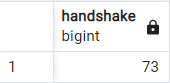
\includegraphics[scale=0.6]{request12.png}}
    \caption{Результат выполнения запроса 12.}
    \label{fig:request12}
\end{figure}

\underline{Запрос 13}. \textbf{Найти книги, названия которых содержат "люб".}
\begin{lstlisting}
    SELECT DISTINCT title FROM books
    WHERE title ~* 'люб'
    \end{lstlisting}

\textbf{Результат} (несколько первых записей) -- Рис. \ref{fig:request13}.

\begin{figure}[ht]
    \center{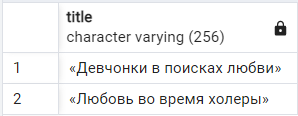
\includegraphics[scale=0.6]{request13.png}}
    \caption{Результат выполнения запроса 13.}
    \label{fig:request13}
\end{figure}

\underline{Запрос 14}. \textbf{Найти книги, названия которых содержат числа.}
\begin{lstlisting}
    SELECT title FROM books
    WHERE title ~ '\d'
    \end{lstlisting}

\textbf{Результат} (несколько первых записей) -- Рис. \ref{fig:request14}.

\begin{figure}[ht]
    \center{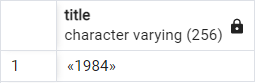
\includegraphics[scale=0.6]{request14.png}}
    \caption{Результат выполнения запроса 14.}
    \label{fig:request14}
\end{figure}

\underline{Запрос 15}. \textbf{Найти первые две книги авторов, которым больше 60 лет.}
\begin{lstlisting}
    WITH d AS (SELECT b.*, row_number() OVER (PARTITION BY first_name, last_name ORDER BY b.release_date) r
    FROM (SELECT b.release_date, a.first_name, a.last_name, b.title
          FROM books b
                   JOIN book_author ba on b.book_id = ba.book_id
                   JOIN authors a on a.author_id = ba.author_id
          WHERE a.year_of_death is not null
            and EXTRACT(epoch FROM a.year_of_death - a.year_of_birth) / (60 * 60 * 24 * 365) > 60) b)
SELECT *
FROM d
WHERE r = 1 OR r = 2;
    \end{lstlisting}

\textbf{Результат} (несколько первых записей) -- Рис. \ref{fig:request15}.

\begin{figure}[ht]
    \center{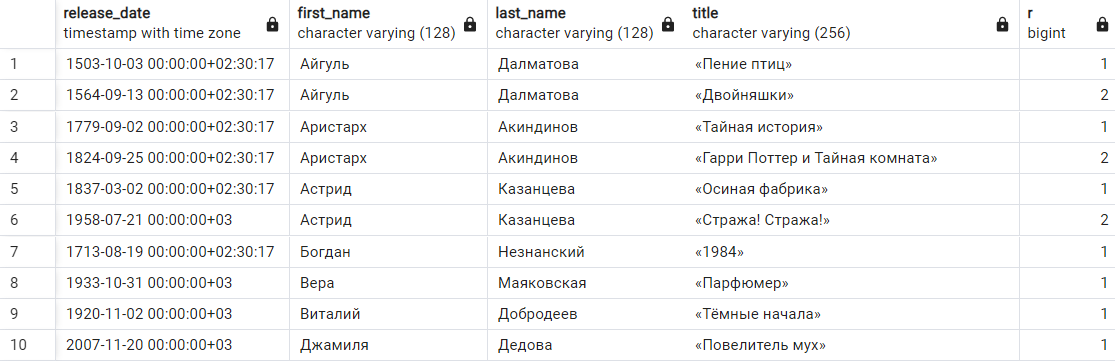
\includegraphics[scale=0.6]{request15.png}}
    \caption{Результат выполнения запроса 15.}
    \label{fig:request15}
\end{figure}


\newpage
\section{Заключение}
Таким образом была спроектирована, создана и заполнена база данных, соответствующая некоторому функционалу книжного сайта \textsl{LiveLib.ru}, а также реализован ряд аналитических запросов к ней.
\end{document}